% !TEX root=../main.tex
\begin{lecture}[Конденсация Бозе-Эйнштейна]
    Мы будем рассматривать Бозе-конденсацию для системы частиц в трехмерном гармоническом потенциале с $\omega_x = \omega_y = \omega_z = 1$.
    \section{Статсумма для системы из нескольких бозе-частиц}
    Для одной частицы мы имели $Z^{\text{single}} = \int dx \rho (x, x, \beta)$.

    Для двух частиц уже берется интеграл по координатам обоих частиц, а матрица плотности $\rho$ уже зависит от координат обоих:
    \begin{align}
        & Z^{\text{two particles}} = \int dx_0 dx_1 \rho (\vec{x}, \vec{x}, \beta) \\
        & \vec{x} = (x_0, x_1)
    \end{align}

    \begin{figure}[ht]
        \begin{subfigure}{0.33\columnwidth}
            \centering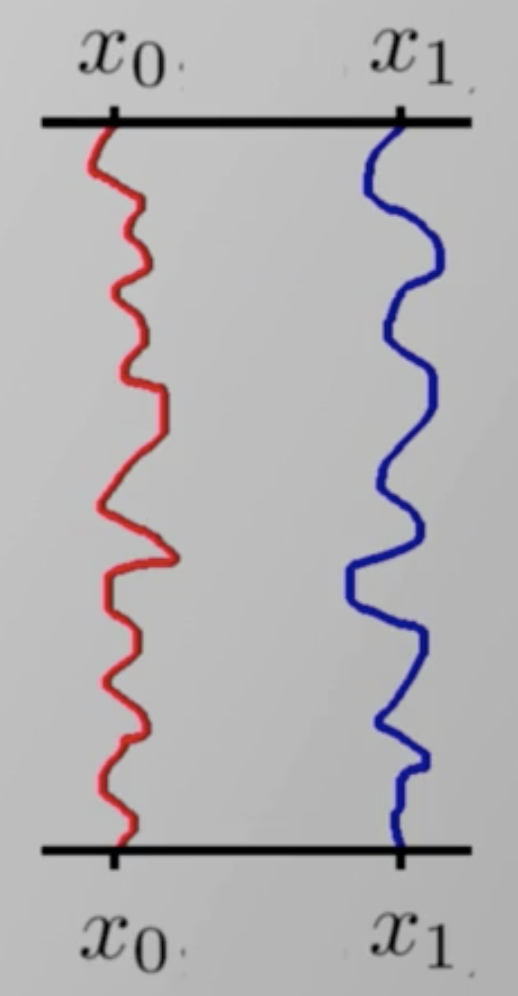
\includegraphics[width=\linewidth]{fig/two-paths-colored}
            \caption{При подсчете путей раздельно по факту получается, что мы считаем их частицы \textit{различимыми}}
            \label{fig:two-paths-colored}
        \end{subfigure}
        \begin{subfigure}{0.66\columnwidth}
            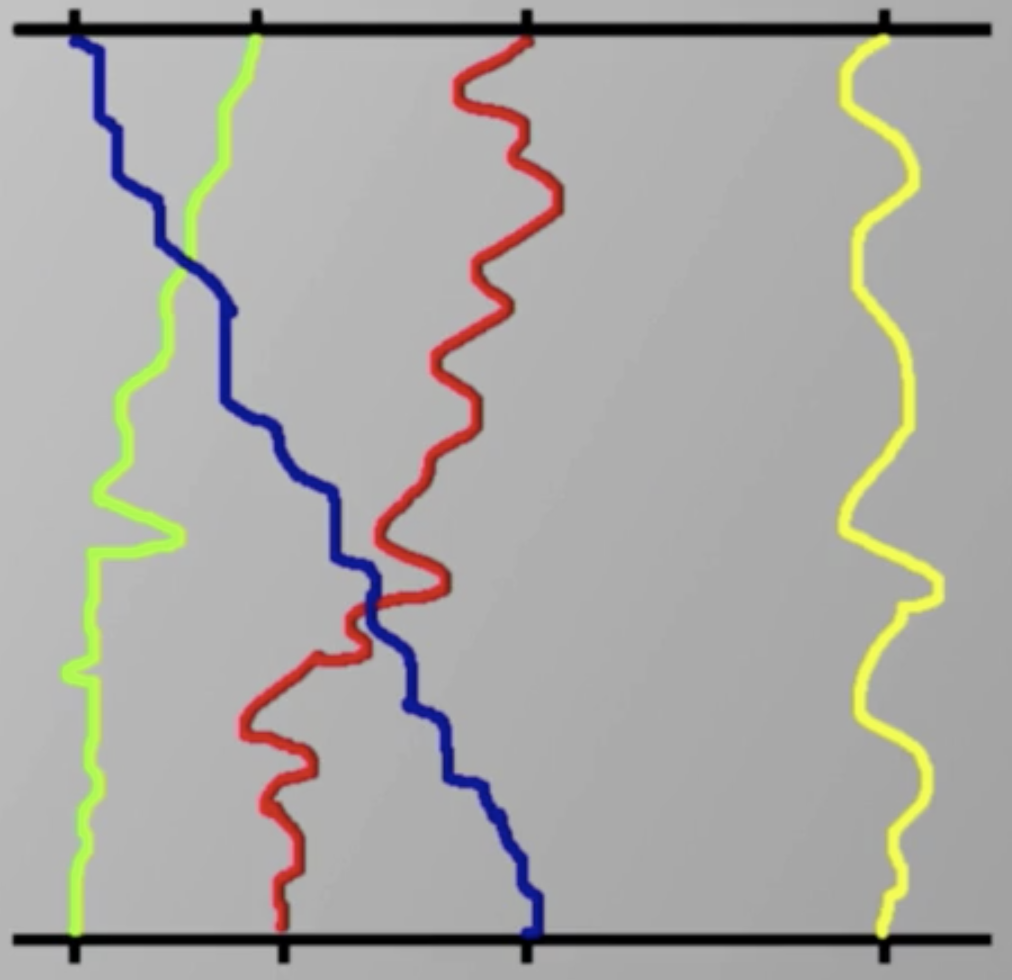
\includegraphics[width=\linewidth]{fig/paths-permutations}
            \caption{Перемешивание путей: частица 1 перешла в частицу 2, частица 3 --- в частицу 1 и т.д.}
            \label{fig:paths-permutations}
        \end{subfigure}
        \caption{Подсчет путей для системы из нескольких частиц}
        % \label{fig:x_k-levy-sampling}
    \end{figure}

    На языке путей это означает, что берется интеграл по двум путям, причем для невзаимодействующих частиц пути независимы, а для взаимодействующих --- как бы \textit{коррелируются} через Trotter decomposition.

    \subsection{Учет неразличимости}

    Однако при таком формализме мы можем раскрасить пути и увидеть, что по факту в своих расчетах мы считаем частицы различимыми.
    Чтобы решить эту проблему, будем брать сумму не только по путям, которые начинаются в $x_1$ и заканчиваются в $x_1$, но и тем, что начинаются в $x_1$ и заканчиваются в другой частице $P(x_1)$.
    Это приводит к правильному выражению статсуммы для такого Path Integral:
    \begin{equation}
        \label{eq:Z_bosons-via-permutations}
        Z^{\text {Bose }} =
        {\color{red} \frac{1}{N!}}
        \int d x_{0} \ldots d x_{N-1}
        {\color{red} \sum_{P}}
        \rho^{\text{distinguishable}}\left(x_{0}, \ldots, x_{N-1} ; x_{P(0)}, \ldots, x_{P(N-1)}, \beta\right)
    \end{equation}

    В случае взаимодействующих частиц нужно разбивать многочастичную $\rho$ на слои (как мы это делали, когда сводили $\beta \rightarrow \beta /N$), а затем применить Trotter decomposition \eqref{eq:trotter-decomposition-definition}.
    Тем не менее, для невзимодействующих частиц матрица плотности факторизуется:
    \begin{equation}
        \label{eq:rho-bosons-ideal-factorized}
        \rho^{\mathrm{ideal}}=\rho\left(x_{0}, x_{P(0)}, \beta\right) \ldots \rho\left(x_{N-1}, x_{P(N-1)}, \beta\right)
    \end{equation}
    Это выражение легко понять: изменение координаты $x_{P(0)}$ или $x_0$ затрагивает только тот кусок, что ответственнен за частицу 0, и никакой другой.
    
    Таким образом, \textit{пути} для свободных частиц \textit{независимы}.

    Заметим, что все рассуждения выше являются общими (за исключением факторизации матрицы плотности для невзимодействующих частиц).

    \section{Алгоритм подсчета статсуммы для системы бозонов}
    При подсчете $Z^{\text{Bose}}$ \eqref{eq:Z_bosons-via-permutations} мы сталкиваемся с двумя проблемами:
    \begin{enumerate}
        \item Сэмплирование перестановок ($\sum\limits_{P}^{} \dots$);
        \item Сэмплирование координат $\{x_i\}$;
    \end{enumerate}

    Рассмотрим их по отдельности.

    \subsection{Простейшее сэмплирование перестановок}
    Для упрощения заменим в выражении статсуммы \eqref{eq:Z_bosons-via-permutations} все члены, зависящие от координат, единицей.
    Это приведет к задаче поиска $N$ перестановок в списке: $Z^{\text{permutation}} = \sum\limits_{P}^{}1$.

    На каждом шаге мы можем менять две частицы (марковский процесс).
    Это отражено в коде \ref{code:permutation_sample}.

    \pythonfile{../w7/programs_lecture_7/permutation_sample}{Подсчет числа перестановок списка из $N$ элементов методом цепей Маркова (\texttt{permutation\_sample.py})}{code:permutation_sample}

    Такой алгоритм корректен: он удовлетворяет условиям detail balance, является irreducible и aperiodic (см. первые недели).

    \subsection{Сведение циклов в перестановках к слоям в Path Integral}

    \begin{wrapfigure}[8]{r}{0.25\linewidth}
        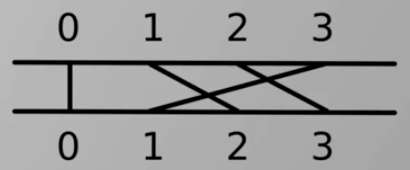
\includegraphics[width=\linewidth]{fig/permutation-cycle}
        \caption{Графическое отображение перестановки $(0)(132)$.}
        \label{fig:permutation-cycle}
    \end{wrapfigure}
    Рассмотрим снова выражение для $Z^{\text{bosons}}$ \eqref{eq:Z_bosons-via-permutations}.
    Возьмем для примера перестановку ${}^{[0, 3, 1, 2]}_{[0, 1, 2, 3]}$ в системе невзаимодействующих частиц.

    Эту перестаноку можно отобразить в виде совокупности двух циклов: $0 \rightarrow 0$ (длина 1) и $1 \rightarrow 3 \rightarrow 2 \rightarrow 1$ (длина 3) --- это изображено на рисунке \ref{fig:permutation-cycle}.
    \textit{Вообще, любую перестановку можно представить в виде комбинации циклов и транспозиций (параллельных переносов). Этот факт можно погуглить.}
    Теперь посмотрим, во что превратится \eqref{eq:Z_bosons-via-permutations} для данной перестановки:
    \begin{align}
        \label{eq:Z_0_132-full}
        & Z_{(0)(132)} = \int dx_0 dx_1 dx_2 dx_3\, \rho(\{x_0, x_1, x_2, x_3\}; \{P(x_0), P(x_1), P(x_2), P(x_3)\}) = \\
        \nonumber
        & \int dx_0\, \rho(x_0, x_0, \beta) \int dx_1 \int dx_2 \int dx_3\, \rho(x_1, {\color{red} x_3}, \beta) \rho({\color{blue} x_2}, x_1, \beta) \rho({\color{red} x_3}, {\color{blue} x_2}, \beta) = \\
        \nonumber
        & \int dx_0 \rho(x_0, x_0, \beta) \int dx_1 \int dx_2 \rho(x_1, x_1, 3\beta)
    \end{align}
Здесь мы воспользовались тем, что $\rho$ для системы невзаимодействующих частиц факторизуется \eqref{eq:rho-bosons-ideal-factorized}, а также свойством конволюции \eqref{eq:rho_convolution-derivation} последовательно несколько раз.

Вот мы и пришли к решению: для интеграла по $x_0$ можно сэмплировать непосредственно из матрицы плотности $\rho^{\text{harmonic}}$ (т.к. мы рассматриваем систему в гармоническом потенциале) при температуре $\beta$.
Для интеграла $x_1$ мы запускаем Lévy path sampling при температуре $3\beta$ и тремя слоями. \textit{Эти матрицы, способ их получения и алгоритм Lévy sampling для гармонического осциллятора были в домашке к неделе 6}.
Точки $x_1, x_2, x_3$ при этом есть промежуточные точки при Lévy sampling с $3\beta$ для гармонического потенциала (см. секцию \ref{sec:levy-harmonic}).

Теперь обобщим это рассуждение.
Для каждой насэмплированной перестановки (как их сэмплировать, будет сказано ниже) мы определяем число циклов и их длину.
Затем для каждой зацикленной координаты составляем соответствующие Path Integral с началом и концом в этой координате, в которых температура будет равна $k\beta$, где $k$ --- длина цикла.
Промежуточные координаты берем из промежуточных точек на слоях в Path Integral (их всегда будет $k$ штук, поскольку соответствующий интеграл берем при температуре $k\beta$).

\textit{Неформально говоря, вся магия здесь держится на том, что циклы в перестановках красиво и аккуратно ложатся на свойство конволюции, что позволяет эффектно сводить циклы с Path Integral по слоям.}

\subsection{Сэмплирование перестановок: алгоритм}

Сэмплируемые таким образом коорданаты имеют zero rejection rate.
Но с другой стороны, нам надо генерить перестановки!
Можно предложить следующий алгоритм:
\begin{enumerate}
    \item Берем начальную перестановку;
    \item Выбираем случайно две частицы и переставляем их;
    \item Считаем вес новой и старой перестановок;
    \item Принимаем с Metropolis acceptance rate: $\frac{\pi_\text{new}}{\pi_\text{old}}$;
\end{enumerate}

Рассмотрим пример.
Возьмем нашу перестановку ${}^{[0, {\color{red} 3}, {\color{blue} 1}, 2]}_{[0, 1, 2, 3]}$ и попробуем в ней переставить 3 и 1 так, что получится перестановка ${}^{[0, {\color{blue} 1}, {\color{red} 3}, 2]}_{[0, 1, 2, 3]}$.
В этом случае
\begin{align*}
    & \pi_\text{old} \propto \rho^{\text{harm}} (x_1, x_3, \beta) \rho^{\text{harm}}(x_2, x_1, \beta) \\
    & \pi_\text{new} \propto \rho^{\text{harm}}(x_1, x_1, \beta) \rho^{\text{harm}}(x_2, x_3, \beta)
\end{align*}
Соответственно, принимаем это изменение с вероятностью $p_\text{acc} (\text{old} \rightarrow \text{new}) = \min\left( 1, \frac{\pi_\text{new}}{\pi_\text{old}}\, \right)$.

\section{Реализация алгоритма}
Следуя идеям из предыдущей секции, можно написать программу \ref{code:markov_harmonic_bosons}.

\pythonfile{../w7/programs_lecture_7/markov_harmonic_bosons}{Бозе-частицы в гармоническом потенциале методом цепей Маркова (\texttt{markov\_harmonic\_bosons.py})}{code:markov_harmonic_bosons}

Обсудим основные моменты.
В алгоритме присутствует два хода: ход частицы и ход перестановки.

Во время хода частицы:
\begin{enumerate}
    \item Выбираем случайную частицу;
    \item Определяем ее цикл перестановок;
    \item Сэмплируем путь Lévy для данного цикла длины $k$;
\end{enumerate}

Во время хода перестановки:
\begin{enumerate}
    \item Выбираем две случайные частицы;
    \item Пытаемся обменять местами их <<партнеров по перестановке>> (частицы, в которые они переходят);
\end{enumerate}

Функция \textit{levy\_harmonic\_path(k, beta)} возвращает координаты Lévy-пути от $0$ до $k\beta$ с $k$ промежуточными слоями.
Функция \textit{rho\_harm(x, xp, beta)} возвращает диагональные и недиагональные элементы матрицы плотности в гармоническом потенциале.

Алгоритм в деталях выглядит следующим образом:
\begin{itemize}
    \item В начале программы (строки 30-32) мы сэмплируем координаты просто из Lévy-пути длиной 1 и пихаем их в словарь \textit{positions}.
    \item Затем выбираем случайную частицу (строка 34) и определяем для нее цикл перестановок (строки 36-40).
    \item Для цикла перестановки мы заново сэмплируем \textbf{все} координаты (строка 42). Чтобы это продолжило быть циклом, мы <<зацикливаем>> новые координаты в словаре \textit{positions} (строки 43-45). Теперь у нас появился новый \textit{путь}, полученный полной заменой одного цикла в уже имеющемся пути. Это был ход частицы.
    \item Из \textbf{всех} позиций частиц, которые когда-либо были созданы алгоритмом, мы выбираем две случайные (строки 46-49), меняем их местами (строки 50-51) и принимаем или отвергаем по алгоритму Метрополиса (строки 52-57).
\end{itemize}

Самое нетривиальное здесь --- это понять, что словарь \textit{positions} постоянно растет: новые сэмплируемые пути не заменяют старые в словаре, а просто добавляются к нему.

\textit{P.S. в Python 2 все словари по-умолчанию есть defaultdict из Python 3. Поэтому приравнивание по ключу создаст запись, если ключа не существует (а не выбросит KeyError).}

При высоких температурах можно обнаружить, что ходы перестановки чаще всего отвергаются (длина циклов $\sim~1$), однако при высоких температурах длина циклов значительно растет (на лекции было $k~\sim~100$).
Это явление --- существенная часть Бозе-конденсации. Если <<выключить>> перестановки в алгоритме (что отражает неразличимость частиц), то явление Бозе-конденсации исчезнет.

\end{lecture}
